\section{Câu 1}
Thiết kế mạch thực hiện hàm: $v_o = 2V_1 + 3V_2 -6V_3$ với yêu cầu chỉ được sử dụng 2 OPAMP.\\
a. Giả sử các OPAMP sử dụng là lí tưởng.\\
b. Giả sử cả 2 OPAMP có $V_{io}=100\mu V, I_{io}=4nA, I_{ib}=18nA$.\\
Tìm ảnh hưởng của điều kiện không lý tưởng của OPAMP lên ngõ ra $V_o$ .\\
\begin{center}
\textbf{Bài giải}
\end{center}
\begin{figure}[H]
	\centering
	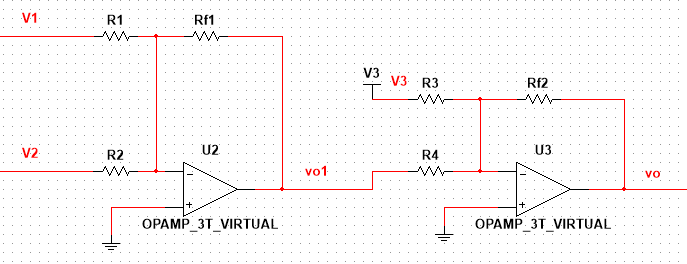
\includegraphics[scale=0.9]{image/C1_a_BT.png}
\end{figure}
a. Ta có:
\[
\left\{
\begin{aligned}
v_{o1} &= -\dfrac{R_{f1}}{R_1}V_1 - \dfrac{R_{f1}}{R_2}V_2 &= -2V_1-3V_2\\
v_o &= -\dfrac{R_{f2}}{R_3}V_3 - \dfrac{R_{f2}}{R4}v_{o1} &= -6V_3-1v_{o1}
\end{aligned}
\right.
\]
Chọn $\boxed{R_{f1}=10K,\; R_{f2}=18K \;\rightarrow\; R_1=5K,\; R_2=3.33K,\; R_3=3K,\; R_4=18K}$
\begin{figure}[H]
	\centering
	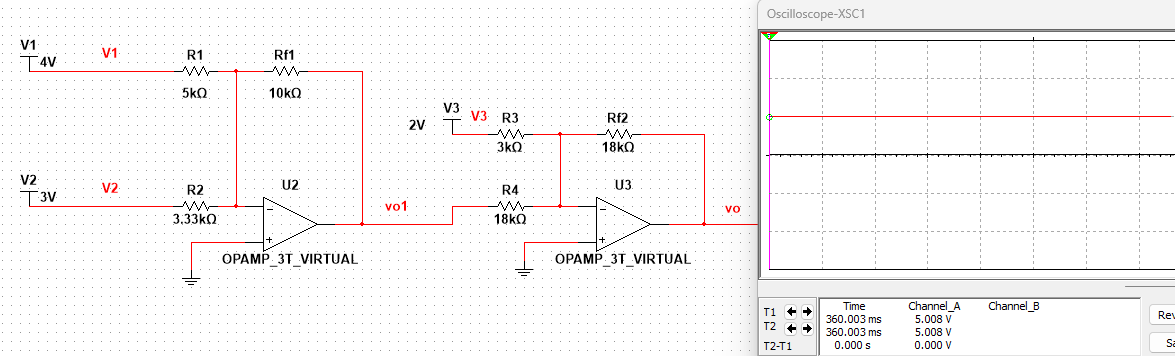
\includegraphics[scale=0.5]{image/C1_simulate.png}
\end{figure}
\textbf{Nhận xét:}\\
- Với $V_1=4V$, $V_2=3V$ ,$V_3=2V$. Theo đề bài, $v_o=5V$ và kết quả mô phỏng được tại $v_o=5.008V$ đúng với yêu cầu thiết kế.\\

b.
